% =====================================================================
% Z3ST one-page handout / leave-behind  --  FEniCS 2026 demo table
% Build:  latexmk -pdf handout.tex   (or  pdflatex handout.tex)
% A4, single page. QR codes via the native 'qrcode' package (no images).
% =====================================================================
\documentclass[11pt]{article}
\usepackage[a4paper,margin=14mm]{geometry}
\usepackage[T1]{fontenc}
\usepackage{helvet}
\renewcommand{\familydefault}{\sfdefault}
\usepackage{xcolor}
\usepackage{graphicx}
\usepackage{animate}   % animated PCMI / damage strip (plays in Adobe; poster=last for print)
\usepackage{tikz}
\usepackage[nolinks]{qrcode}
\usepackage{enumitem}
\usepackage{microtype}
\pagestyle{empty}
\setlength{\parindent}{0pt}

\definecolor{z3blue}{HTML}{1F6FB2}
\definecolor{z3teal}{HTML}{2A9D8F}
\definecolor{z3amber}{HTML}{E9A23B}
\definecolor{z3ink}{HTML}{23303A}
\definecolor{z3soft}{HTML}{EEF2F5}
\color{z3ink}

\newcommand{\qrcard}[3]{% url, label, sub
  \begin{minipage}[t]{0.30\linewidth}\centering
    \qrcode[height=2.5cm]{#1}\\[2pt]
    {\color{z3blue}\bfseries #2}\\
    {\footnotesize\color{z3ink!70} #3}
  \end{minipage}}

\begin{document}

% ---- header band ----------------------------------------------------
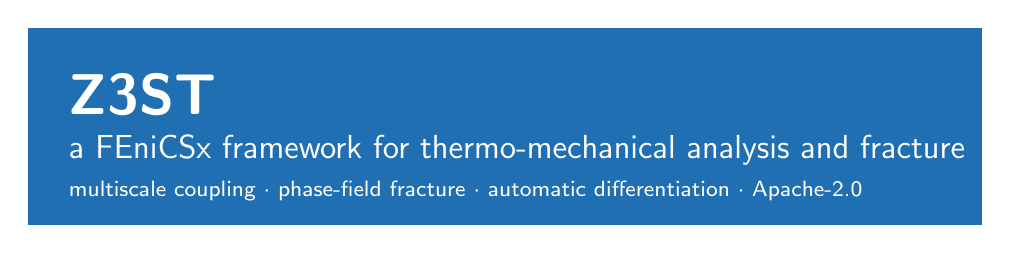
\begin{tikzpicture}
  \fill[z3blue] (0,0) rectangle (\linewidth,2.5cm);
  \node[anchor=west,text=white] at (0.4,1.65)
    {\fontsize{20}{22}\selectfont\bfseries Z3ST};
  \node[anchor=west,text=white] at (0.4,0.95)
    {\large a FEniCSx framework for thermo-mechanical analysis and fracture};
  \node[anchor=west,text=white] at (0.4,0.42)
    {\footnotesize multiscale coupling $\cdot$ phase-field fracture $\cdot$ automatic differentiation $\cdot$ Apache-2.0};
\end{tikzpicture}

\vspace{4mm}

% ---- two columns ----------------------------------------------------
\begin{minipage}[t]{0.56\linewidth}
  {\large\bfseries Write the energy. Get everything else.}\\[2mm]
  Constitutive models are entered as a strain-energy density. UFL's automatic
  differentiation produces the stress and the consistent tangent --- you never
  hand-derive a Jacobian.

  \vspace{2mm}
  \colorbox{z3soft}{\parbox{\linewidth}{\ttfamily\small
  \textcolor{z3blue}{P}\ \ = ufl.diff(psi, F)\hfill\textcolor{z3ink!60}{\# 1st Piola--Kirchhoff}\\
  \textcolor{z3blue}{Jac} = ufl.derivative(R, u)\hfill\textcolor{z3ink!60}{\# tangent, also AD}}}

  \vspace{3mm}
  {\bfseries What it does}
  \begin{itemize}[leftmargin=4mm,itemsep=1pt,topsep=2pt]
    \item coupled thermo-mechanics, staggered with adaptive relaxation
    \item elasticity, hyperelasticity, J2 plasticity, phase-field damage (AT1/AT2)
    \item multiscale: cluster dynamics, fracture length scale, gap conductance
    \item one driver, regimes \texttt{1D/2D/3D/axisymmetric/plane-stress}
    \item materials and cases are YAML; verified by $\sim$50 non-regression checks (a subset re-run in CI)
  \end{itemize}

  \vspace{2mm}
  {\bfseries Run it}\\[1mm]
  {\ttfamily\small conda activate z3st\\ python -m z3st\ \ \ \textcolor{z3ink!60}{\# reads input.yaml}}
\end{minipage}\hfill
\begin{minipage}[t]{0.40\linewidth}
  \centering
  % animations play in Adobe Reader / pdfpc; poster=last shows the
  % fully-developed final frame in print / static viewers.
  \fbox{\animategraphics[autoplay,loop,poster=last,width=\linewidth]{7}%
    {../oral/figures/anim_pcmi/frame_}{0}{38}}\\[1mm]
  {\footnotesize\color{z3ink!75} PCMI over a full irradiation: the gap closes,
  contact pressure builds, and peak fuel $T$ drops as conductance recovers.}\\[2.5mm]
  \fbox{\animategraphics[autoplay,loop,poster=last,width=\linewidth]{9}%
    {../oral/figures/anim_damage/frame_}{0}{50}}\\[1mm]
  {\footnotesize\color{z3ink!75} UO\textsubscript{2} pellet thermal-shock cracking:
  fully coupled temperature $\to$ elastic strain $\to$ phase-field damage. A 2D
  plane-strain reproducer of McClenny et al. (JNM 2022).}\\[1mm]
  {\scriptsize\color{z3ink!55}\itshape animated in Adobe Reader / pdfpc}
\end{minipage}

\vspace{5mm}
\textcolor{z3amber}{\rule{\linewidth}{1.4pt}}
\vspace{3mm}

% ---- QR row ---------------------------------------------------------
\begin{center}
  \qrcard{https://github.com/giozu/z3st}{code}{github.com/giozu/z3st}\hfill
  \qrcard{https://giozu.github.io/z3st/}{docs}{giozu.github.io/z3st}\hfill
  \qrcard{https://doi.org/10.5281/zenodo.17748028}{cite}{doi 10.5281/zenodo.17748028}
\end{center}

\vfill
\begin{center}\footnotesize\color{z3ink!75}
  Giovanni Zullo (presenter) $\cdot$ Giovanni Nicodemo $\cdot$ Elisa Cappellari $\cdot$
  Davide Pizzocri $\cdot$ Lelio Luzzi\\[1pt]
  Politecnico di Milano $\cdot$ giovanni.zullo@polimi.it
  \hfill FEniCS 2026 $\cdot$ live software demonstration --- come and run it with me
\end{center}

\end{document}
